\chapter{Calculus of variations}
\label{chap:CalculusVariation}
The calculus of variations is fundamental in understanding the principles of analytic mechanics. The main problems to be considered are those of finding stationary values of functions and of integrals. Technically, the analysis of stationary values of functions is called ``calculus'', while that of integrals is called ``calculus of variations''

\section{Virtual displacement}
The calculus of variations deals with ``virtual'' displacements, rather than ``differential'' displacements, and ``variations of functions''. For example, when considering the time-evolution of some coordinate, $q(t)$, one can  write the differential, $dq$, which is a measure of the infinitesimal change in $q$ for a given change, $dt$, in time. 

A virtual displacement, denoted $\delta q$, is a change in $q(t)$, without the corresponding change in time. That is, the value of $q(t)$ is infinitesimally displaced from the value that it should have at a particular time. In some respects, this is an un-physical change in $q$.

As will be seen later, it is very useful to look at these un-physical changes in quantities to set restriction on how they can change physically, thus determining their equations of motion. Another example is the potential energy of a marble at the bottom of the bowl; it may be interesting for us to consider how the potential energy would change if the marble were to be (un-physically) displaced horizontally away from the bottom of the bowl. Those considerations will lead us to understanding how the marble can behave physically.

\section{Variation of a function}
Consider a function, $y=f(x)$, and a new function, $\bar{f}(x)$:
\begin{align}
\bar{f}(x)=f(x)+\epsilon \phi(x)
\end{align}
where $\epsilon$ is a number that we can make arbitrarily small, and $\phi(x)$ is a function that is continuous and differentiable in some interval $x=a\dots b$ over which $f(x)$ is defined, continuous and differentiable. We define the variation of a function as:
\begin{align}
\label{eqn:vardef}
\delta y \equiv \bar{f}(x) -f(x) = \epsilon \phi(x)
\end{align}
The change in $f(x)$ is infinitesimal and ``virtual'', meaning that we can choose any arbitrary well behaved $\phi(x)$. Thus $\delta y$ does not represent a ``real'' change in the function from a change in its dependent variables. Again, note the difference between $\delta y$ and $dy$; $dy$ is the (familiar) change in $f(x)$ from a corresponding change in $x$ by $dx$, while $\delta y$ is a change in $f(x)$ \textbf{without} a change in $x$, and is a \textbf{new} function. This is illustrated in Figure \ref{fig:VirtualDisplacement}.
\begin{figure}[!h]
\center
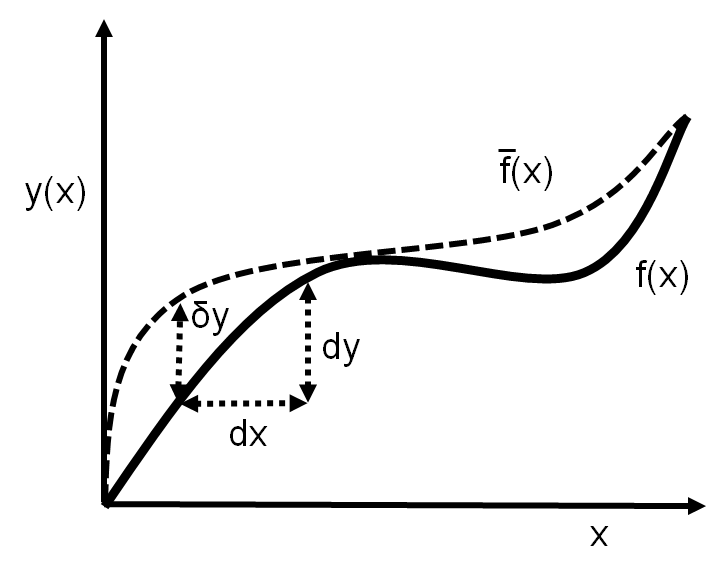
\includegraphics[width=0.5\textwidth]{figures/VirtualDisplacement.png}
\caption{\label{fig:VirtualDisplacement}A function $y=f(x)$ showing a differential change $dx$ which corresponds to a change in $x$ of $dx$. The variation of the function at a point, $\delta y$, is also shown, which is independent of a change in $x$ and leads to a different function, $\bar{f}(x)$.}
\end{figure}
For the calculus of variations, we only consider changes in the dependent variables, thus:
\begin{align}
\delta x = 0
\end{align}

\subsection{Properties of the $\delta$ operator}
\subsubsection{Commutation with differentiation}
Consider the ``derivative of the variation'':
\begin{align}
\frac{d}{dx}\delta y =\frac{d}{dx} \left[\bar{f}(x)-f(x) \right]=\frac{d}{dx} \epsilon \phi(x)=\epsilon \phi'(x)
\end{align}
where we have used an apostrophe (') to designate derivatives with respect to $x$. Now consider the ``variation of the derivative'':
\begin{align}
\delta \left(\frac{d}{dx}f(x)\right) \equiv \frac{d\bar{f}}{dx}-\frac{df}{dx} = \frac{d}{dx} (f(x)+\epsilon \phi(x)) - \frac{df}{dx} = \epsilon \phi'(x)
\end{align}
We thus find that $\delta$ is commutative with $\frac{d}{dx}$:
\begin{align}
\label{eqn:vardiffcommut}
\therefore \delta \left(\frac{dy}{dx}\right) = \frac{d}{dx}\left(\delta y\right)
\end{align}
\subsubsection{Commutation with integration}
Next, consider the variation of a definite integral:
\begin{align}
\delta \int_a^b f(x) dx &\equiv  \int_a^b \bar{f}(x) dx - \int_a^b f(x) dx = \int_a^b (\bar{f}(x)-f(x)) dx\nonumber\\
\therefore \delta \int_a^b f(x) dx &= \int_a^b \delta f(x) dx 
\end{align}
The delta operator also commutes with respect to integration.
\subsubsection{Chain Rule}
If $y$ is a function of $x$, the variation of a function, $F(y)$, is given by:
\begin{align}
\delta F(y) &= F(y+\delta y)-F(y)
\end{align}
We can expand $F(y+\delta y)$ using a Taylor series, where $\delta y$ is small:
\begin{align}
F(y+\delta y)=F(y)+\frac{dF}{dy}\delta y + \frac{1}{2!}\frac{d^2F}{dy^2}(\delta y)^2+\dots 
\end{align}
Given that $\delta y$ are small, we can ignore the terms in powers higher than 2:
\begin{align}
F(y+\delta y)&=F(y)+\frac{dF}{dy}\delta y\nonumber\\
\therefore \delta F(y)&=\frac{dF}{dy}\delta y
\label{eqn:varChainRule}
\end{align}
which is (like) the Chain Rule.
\begin{example}{0pt}{Determine $\delta(\cos{\theta})$}{}
Using the Chain Rule:
\begin{align*}
\delta(\cos{\theta})=-\sin{\theta}\delta\theta
\end{align*}
\end{example}
\noindent
If the function $F$ is a function of multiple functions, $y(x), z(x), \dots$, we proceed the same way, but using partial derivatives:
\begin{align}
\delta F(y,z,\dots) &= F(y+\delta y, z+\delta z, \dots)-F(y,z,\dots)\nonumber\\
&=\frac{\partial F}{\partial y}\delta y +\frac{\partial F}{\partial z}\delta z+\dots+ \frac{1}{2!}\left(\frac{\partial^2F}{\partial y}\delta^2y+\frac{\partial^2F}{\partial z}\delta^2z+2\frac{\partial^2 F}{\partial y\partial z}\delta y \delta z+\dots \right) +\dots
\label{eqn:varChainRuleMulti}
\end{align}
where again, we will neglect the terms in $\delta^2$ and higher.
\begin{example}{0pt}{Compare the differential displacement and virtual displacement of a position vector $\vec{r}=\vec{r}(q_1,q_2,\dots,q_n,t)$ that is a function of generalized coordinates, $q$.}{}
When considering the position of a particle as a function of the generalized coordinates:
\begin{align*}
\vec{r}=\vec{r}(q_1,q_2,\dots,q_n,t)
\end{align*}
the differential displacement (also the ``true'' displacement):
\begin{align*}
d\vec{r}=\frac{\partial\vec{r}}{\partial q_1}dq_1+\dots+\frac{\partial\vec{r}}{\partial q_n}dq_n+\frac{\partial\vec{r}}{\partial t}dt
\end{align*}
whereas the virtual displacement does not have a time differential in it:
\begin{align*}
\delta\vec{r}=\frac{\partial\vec{r}}{\partial q_1}\delta q_1+\dots+\frac{\partial\vec{r}}{\partial q_{n}}\delta q_{n}
\end{align*}
\end{example}

\section{Stationary value of a function}
In analytic mechanics, we will be interested in the stationary value of an integral. We start by considering the stationary value of a function. For example, an n-dimensional function $F(q_1, q_2, \dots, q_n)$, can be pictured as a surface in a space with n+1 dimension (for example, imagine a 2-dimensional surface in 3-dimensional space). The stationary points of the functions are locations where the surface is ``flat'', and can correspond to local ``extrema'' (minima or maxima) or ``saddle points''. We can use the formalism of variations to find the conditions for such points. 

If the point, $P$, is a stationary value of the function, $F(q_1, q_2, \dots, q_n)$, then, the variation of the function near $P$ in the direction of an arbitrary virtual displacement, $\delta\vec{q}$, is 0 (the function is flat in the infinitesimal region near the point). The variation of the function is (technically called the ``first variation'', as we drop the higher order terms in the Taylor series):
\begin{align}
\delta F&=\frac{\partial F}{\partial q_1}\delta q_1 + \frac{\partial F}{\partial q_2}\delta q_2 +\dots+\frac{\partial F}{\partial q_N}\delta q_N
\end{align}  
We can write this in terms of finite numbers if we write the virtual displacements as:
\begin{align}
\delta q_i=\epsilon \alpha_i
\end{align}
where $\vec{\alpha}$ is a vector in the direction of the virtual displacement and $\epsilon$ is a number that tends to zero. The rate of change of the function, $F$, in the direction of $\vec{\alpha}$ is:
\begin{align}
\frac{\delta F}{\epsilon}=\frac{\partial F}{\partial q_1}\alpha_1 + \frac{\partial F}{\partial q_2}\alpha_2 +\dots+\frac{\partial F}{\partial q_N}\alpha_N
\end{align} 
which must vanish for a stationary point (writing the above equation as a sum):
\begin{align}
\sum_i\frac{\partial F}{\partial q_i}\alpha_i =0
\end{align} 
In order to have a stationary point, the rate of the change of the function must vanish for any direction, $\vec{\alpha}$, so that each term must be equal to zero, independent of the $\alpha_i$:
\begin{align}
\frac{\partial F}{\partial q_i}\alpha_i &=0\nonumber\\
\therefore \frac{\partial F}{\partial q_i}&=0
\end{align}
and we recover the familiar result from calculus that the partial derivatives must vanish at $P$, for that point to be a stationary point of the function. The second order derivatives (``second variations'') are needed in order to know if this is a local minimum, maximum or saddle point. For analytic mechanics, we will generally only need to know if the point is stationary.

\section{Constraints and Lagrange multipliers}
\subsection{Single constraint}
In some cases, the problem of finding a stationary point does not generalize to any virtual displacement, as constraints between coordinates limit the choice of direction for $\vec{\alpha}$. For example, in the case finding the minimum of the potential energy of a marble in a bowl, we would have a constraint equation in the form:
\begin{align}
x^2+y^2+z^2=(R-r)^2
\end{align}
where $(x,y,z)$ are the position of the center of mass of the ball, $R$ is the radius of the bowl, and $r$ is the radius of the ball. The ball is constrained to be in the bowl, so we cannot just consider any point in space as the minimum of the potential energy.

In general then, we seek to minimize the function $F(q_1, q_2, \dots, q_n)$, subject to some constraint equation(s) between the coordinates:
\begin{align}
f(q_1, q_2, \dots, q_n)=0
\end{align}
The obvious (and valid) way to handle this is to use the constraint equation to eliminate one of the variables from $F$ and work with n-1 independent (generalized) coordinates. However, it may not be convenient to eliminate a coordinate, and there might not be an obvious choice of which coordinate should be the ``dependent'' one. Lagrange's method of multipliers allows one to preserve all the coordinates while including the constraints (or ``auxiliary conditions''). We start by finding the stationary point subject to a single auxiliary condition. We have:
\begin{align}
\delta f=\frac{\partial f}{\partial q_1}\delta q_1 + \frac{\partial f}{\partial q_2}\delta q_2 +\dots+\frac{\partial f}{\partial q_n}\delta q_n=0
\end{align}
In order to have a stationary point of $F$, we also have:
\begin{align}
\delta F=\frac{\partial F}{\partial q_1}\delta q_1 + \frac{\partial F}{\partial q_2}\delta q_2 +\dots+\frac{\partial F}{\partial q_n}\delta q_n=0
\end{align}
however, unlike in the un-constrained case, the $\delta q_i$, are not independent, thus this no longer implies that each term (and hence each partial derivative) is zero. Since the two above equations are zero, we can create a linear combination of them, which will still equal zero:
\begin{align}
&\delta F+\lambda \delta f=\frac{\partial F}{\partial q_1}\delta q_1 + \frac{\partial F}{\partial q_2}\delta q_2 +\dots+\frac{\partial F}{\partial q_n}\delta q_n + \lambda (\frac{\partial f}{\partial q_1}\delta q_1 + \frac{\partial f}{\partial q_2}\delta q_2 +\dots+\frac{\partial f}{\partial q_n}\delta q_n)=0\nonumber\\
&\sum_{i=1}^{n} \left(\frac{\partial F}{\partial q_i}+ \lambda \frac{\partial f}{\partial q_i}\right)\delta q_i=0
\end{align}
where $\lambda$ is called a ``Lagrange multiplier'', and is not known a priori. Note again that only the sum is zero, not the individual terms. We now \textbf{choose} $\lambda$ so that the n-th term is zero:
\begin{align}
\frac{\partial F}{\partial q_n}+ \lambda \frac{\partial f}{\partial q_n}=0
\end{align}
Given the chosen value of $\lambda$, the sum now contains one less term:
\begin{align}
\sum_{i=1}^{n-1} \left(\frac{\partial F}{\partial q_i}+ \lambda \frac{\partial f}{\partial q_i}\right)\delta q_i&=0
\end{align}
At this point however, we effectively imposed the constraint to eliminate $\delta q_n$; the remaining coordinates can now be varied independently (``freely''), so that the remaining terms (given $\lambda$) are individually zero:
\begin{align}
\frac{\partial F}{\partial q_i}+ \lambda \frac{\partial f}{\partial q_i}=0 \text{       (i=1, 2, \dots n-1)}
\end{align}
We thus have $n-1$ equations as above, and 1 equation to determine $\lambda$, resulting in $n$ equations to find the point where $F$ is stationary given the auxiliary condition $f=0$. By inspection, those equations are the same and the distinction between dependent and independent variables vanishes!

This method can thus be written a little bit more generally by considering all the $\delta q_i$ as independent instead of (artificially) eliminating $\delta q_n$, and considering the variation:
\begin{align}
\delta F + \lambda \delta f
\end{align}
We have:
\begin{align}
\delta (F+\lambda f) &= \delta F+ (\delta \lambda) f + \lambda (\delta f\nonumber)\\
&=\delta F + \lambda \delta f
\end{align}
since $f=0$. We can then construct a new function, $\bar{F}$:
\begin{align}
\bar{F}=F + \lambda f
\end{align}
and consider the stationary points of $\bar{F}$ without having to worry about auxiliary conditions, thus treating all variations of the coordinates as unconstrained (``free variations''). In this situation, we have n equations by setting the partial derivatives of $\bar{F}$ to zero and 1 equation from the constraint equation $f=0$. This allows us to solve for the $n$ values of $q$ at the minimum and the unknown $\lambda$.

\begin{example}{0pt}{Calculate the dimensions, $x,y,z$ of a box that maximizes the volume for a fixed surface area of 2A.}{}
We wish to maximize the volume of a box, given by:
\begin{align*}
F(x,y,z)=xyz
\end{align*}
subject to the constraint that the area is equal to 2A:
\begin{align*}
2xy+2xz+2yz=2A
\end{align*}
Therefore, the constraint can be written as:
\begin{align*}
f(x,y,z)=xy+xz+yz-A=0
\end{align*}
We thus introduce a Lagrange multiplier, $\lambda$, and minimize
\begin{align*}
\bar{F}=F+\lambda f= xyz+\lambda(xy+xz+yz-A)
\end{align*}
This gives us the 3 equations (one for each coordinate):
\begin{align*}
\frac{\partial \bar{F}}{\partial x}&=yz+\lambda(y+z)=0\\
\frac{\partial \bar{F}}{\partial y}&=xz+\lambda(x+z)=0\\
\frac{\partial \bar{F}}{\partial z}&=yx+\lambda(y+x)=0
\end{align*}
Together with the constraint equation, this gives 4 equations and 4 unknowns ($x,y,z,\lambda$). We can multiply each of the 3 equations by $x,y,z$ respectively to obtain:
\begin{align*}
xyz+x\lambda(y+z)=0\\
yxz+y\lambda(x+z)=0\\
zyx+z\lambda(y+x)=0
\end{align*}
From the first two equations:
\begin{align*}
\therefore x\lambda(y+z)=y\lambda(x+z)\\
\lambda x= \lambda y
\end{align*}
giving us the possibility that either $\lambda=0$ or $x=y$. If $\lambda=0$ anyone of the above equations imply that $xyz=0$, which corresponds to a volume of zero. In principle, our method will only give us a stationary value, and a volume of zero is indeed a minimum of the volume. However, that is not the choice of interest for us, so we choose $x=y$. Combining the other two equations gives us that $x=z$, showing us that the result is a cube. We can use the constraint equations to find the dimensions of the cube:
\begin{align*}
f(x,y,z)=xy+xz+yz-A=3x^2-A=0\nonumber\\
\therefore x=\sqrt{\frac{A}{3}}
\end{align*}
We found our solution and did not need to explicitly solve for the Lagrangian multiplier. Also note that our volume function itself has no maximum, however, the auxiliary condition results in a stationary value that is other than the minimum.
\label{ex:boxvolume}
\end{example}


\subsection{Multiple constraints}
The treatment is similar when we have multiple auxiliary conditions (say $k$ such constraints):
\begin{align}
f_1(q_1, q_2, \dots, q_n)&=0\nonumber\\
f_2(q_1, q_2, \dots, q_n)&=0\nonumber\\
\dots\nonumber\\
f_k(q_1, q_2, \dots, q_n)&=0
\end{align}
where we now have $n-k$ degrees of freedom. The variation of the auxiliary conditions are:
\begin{align}
\delta f_i=\frac{\partial f_i}{\partial q_1}\delta q_1 + \frac{\partial f_i}{\partial q_2}\delta q_2 +\dots+\frac{\partial f_i}{\partial q_n}\delta q_n=0
\end{align}
Again, we wish to find the stationary point of $F$, leading to:
\begin{align}
\delta F = \sum_{i=1}^{n}\frac{\partial F}{\partial q_i}\delta q_i=0
\end{align}
We now introduce a Lagrange multiplier $\lambda_i$ for each of the $k$ auxiliary conditions $f_i$, so that the following linear combination is still zero:
\begin{align}
\label{eqn:multilagrangemulti}
\delta F + \lambda_1 \delta f_1 +\lambda_2 \delta f_2 +\dots+\lambda_k \delta f_k&=0\nonumber\\
\sum_{i=1}^{n}\left(\frac{\partial F}{\partial q_i}+\lambda_1 \frac{\partial f_1}{\partial q_i}+\dots +\lambda_k \frac{\partial f_k}{\partial q_i}\right)\delta q_i=0
\end{align}
We now choose to solve for the $k$ Lagrange multipliers by eliminating the last $k$ terms in the sum, leading to $k$ equations for the $k$ unknown $\lambda$:
\begin{align}
\label{eqn:multilagrangemulti2}
&\frac{\partial F}{\partial q_n}+\lambda_1 \frac{\partial f_1}{\partial q_n}+\dots +\lambda_k \frac{\partial f_k}{\partial q_n}=0\nonumber\\
&\frac{\partial F}{\partial q_{n-1}}+\lambda_1 \frac{\partial f_1}{\partial q_{n-1}}+\dots +\lambda_k \frac{\partial f_k}{\partial q_{n-1}}=0\nonumber\\
&\frac{\partial F}{\partial q_{n-2}}+\lambda_1 \frac{\partial f_1}{\partial q_{n-2}}+\dots +\lambda_k \frac{\partial f_k}{\partial q_{n-2}}=0\nonumber\\
&\dots \nonumber\\
&\frac{\partial F}{\partial q_{n-k+1}}+\lambda_1 \frac{\partial f_1}{\partial q_{n-k+1}}+\dots +\lambda_k \frac{\partial f_k}{\partial q_{n-k+1}}=0
\end{align}
The rest of the $n-k$ coordinates in equation \ref{eqn:multilagrangemulti} can now be varied freely, so that each corresponding terms in the sum must vanish:
\begin{align}
\sum_{i=1}^{n-k}\left(\frac{\partial F}{\partial q_i}+\lambda_1 \frac{\partial f_1}{\partial q_i}+\dots +\lambda_k \frac{\partial f_k}{\partial q_i}\right)\delta q_i=0
\end{align}
thus giving us $n-k$ equations:
\begin{align}
&\frac{\partial F}{\partial q_1}+\lambda_1 \frac{\partial f_1}{\partial q_1}+\dots +\lambda_k \frac{\partial f_k}{\partial q_1}=0\nonumber\\
&\frac{\partial F}{\partial q_2}+\lambda_1 \frac{\partial f_1}{\partial q_2}+\dots +\lambda_k \frac{\partial f_k}{\partial q_2}=0\nonumber\\
&\dots \nonumber\\
&\frac{\partial F}{\partial q_{n-k}}+\lambda_1 \frac{\partial f_1}{\partial q_{n-k}}+\dots +\lambda_k \frac{\partial f_k}{\partial q_{n-k}}=0
\end{align}
Again, by inspection, these equations are the same as those in equation \ref{eqn:multilagrangemulti2}, removing any distinction between dependent and independent variables. We can thus construct the function $\bar{F}$:
\begin{align}
\bar{F}=F+\lambda_1 f_1+\lambda_2 f_2 +\dots +\lambda_k f_k
\end{align}
and treat all of the coordinates in the same way. That is, instead of performing the variation of $F$ subject to the auxiliary conditions, we can perform the variation on $\bar{F}$ and ``ignore'' the auxiliary conditions. This gives us the $n$ equations:
\begin{align}
\frac{\partial F}{\partial q_i}+\lambda_1 \frac{\partial f_i}{\partial q_i}+\dots +\lambda_k \frac{\partial f_k}{\partial q_i}=0 \text{        (i=0\dots n)}
\end{align}
together with the $k$ constraint equations to determine the $n$ coordinates $q_i$ and the $k$ Lagrange multipliers.
\section{Stationary value of an integral}
In analytic mechanics, we will find that we need to find the stationary value of an integral. For example, we may need to find the curve $y(x)$ that results in the definite integral of some function $L(y,y',x)$ being maximized (or stationary). We called the definite integral, $I$, a ``functional'':
\begin{align}
I = \int_a^b L(y,y',x)dx
\end{align}
One common example is the ``Brachistochrone'' problem, in which we wish to find the shape of a wire, $y(x)$, that minimizes the time for a frictionless bead to slide down under gravity from some point $a$ to another point $b$. This problem in fact led to the development of the field of variational calculus.
\begin{example}{0pt}{Derive the functional corresponding to a bead sliding under gravity down a frictionless wire given by the function $y(x)$}{\capfig{0.3\textwidth}{figures/bchrone.png}{Bead sliding under gravity on a wire from a to b.}}
The time that it takes to slide down the path is given by the integral of the time it takes to slide down an infinitesimal arc, $ds$:
\begin{align*}
T=\int_a^b \frac{ds}{v}
\end{align*}
where v is the instantaneous speed. The speed is easily found by conservation of energy. If the bead started at rest:
\begin{align*}
\frac{1}{2}mv^2=mg(y_a-y)\nonumber\\
\therefore v =\sqrt{2g(y_a-y)}
\end{align*}
The arc-length, $ds$, can be expressed in terms of $dx$ and $dy$:
\begin{align*}
ds=\sqrt{dx^2+dy^2}=\sqrt{1+y'^2}dx
\end{align*}
Finally, the time is given by:
\begin{align*}
T=\int_a^b \frac{\sqrt{1+y'^2}}{\sqrt{2g(y_a-y)}}dx
\end{align*}
And the problem is that of solving for the function $y(x)$ that minimizes the ``functional'' $T$, given by the definite integral of $L(y,y',x)$, where:
\begin{align*}
L(y,y',x)=\frac{\sqrt{1+y'^2}}{\sqrt{2g(y_a-y)}}
\end{align*}
\label{ex:brach}
\end{example}
\noindent
We thus want to find the condition on $L$ such that the functional, $I$, is stationary, given the boundary condition that the function, $y(x)$, passes through $a$ and $b$.

\noindent
In analogy with finding the stationary point of a function, we examine the rate of change of the functional as we vary $y(x)$. We start with the variation of the integrand:
\begin{align}
\delta L(y,y',x)=L(y+\delta y, y'+\delta y', x)-L(y,y',x)
\end{align}
where, as you recall, we do not consider any variations in $x$. We can use the first order terms in $\delta$ from a Taylor series to expand $L(y+\delta y, y'+\delta y', x)$:
\begin{align}
L(y+\delta y, y'+\delta y', x)=L(y,y',x)+\frac{\partial L}{\partial y}\delta y+\frac{\partial L}{\partial y'}\delta y'
\end{align}
Thus:
\begin{align}
\delta I &= \delta \int_a^b L(y,y',x)dx\nonumber\\
&= \int_a^b \delta L(y,y',x)dx\nonumber\\
&= \int_a^b  \left( \frac{\partial L}{\partial y}\delta y+\frac{\partial L}{\partial y'}\delta y'\right)dx
\end{align}
Recalling from equations \ref{eqn:vardef} and \ref{eqn:vardiffcommut}  that we can write:
\begin{align}
\delta y = \epsilon \phi(x)\nonumber\\
\delta y' = \epsilon \phi'(x)
\end{align}
where $\phi(x)$ is a small variation of the function $y(x)$. The functional becomes:
\begin{align}
\delta I &=\epsilon \int_a^b  \left( \frac{\partial L}{\partial y}\phi(x)+\frac{\partial L}{\partial y'}\phi'(x)\right)dx
\end{align}
Now, since we want to find a stationary value of $I$, we require the rate of change of $\delta I$ with respect to $\epsilon$ to be zero:
\begin{align}
\frac{d\delta I}{d\epsilon}=\frac{\delta I}{\epsilon} &=\int_a^b  \left( \frac{\partial L}{\partial y}\phi(x)+\frac{\partial L}{\partial y'}\phi'(x)\right)dx=0
\end{align}
The second part can be integrated by parts:
\begin{align}
\int_a^b \frac{\partial L}{\partial y'}\phi'(x)dx=\phi(x)\frac{\partial L}{\partial y'}\Big |_a^b-\int_a^b \frac{d}{dx}\left(\frac{\partial L}{\partial y'}\right)\phi(x)dx
\end{align}
The first term of integration by parts is zero, because the function $y(x)$ is fixed at the end points of the integration range, so $\phi(x=a)=\phi(x=b)=0$. We thus have:
\begin{align}
\frac{\delta I}{\epsilon} &=\int_a^b  \left( \frac{\partial L}{\partial y}\phi(x)-\frac{d}{dx}\left(\frac{\partial L}{\partial y'}\right)\phi(x)\right)dx\nonumber\\
&=\int_a^b  \phi(x)\left( \frac{\partial L}{\partial y}-\frac{d}{dx}\left(\frac{\partial L}{\partial y'}\right)\right)dx=0
\label{eqn:ELderiv}
\end{align}
The only way for this integral to vanish, regardless of the choice of $\phi(x)$ is for the remaining part of the integrand to always be zero. This leads to the ``Euler-Lagrange'' equation, which is the condition for the functional $\int L(y,y',x)dx$ to be stationary:
\begin{align}
\frac{d}{dx}\left(\frac{\partial L}{\partial y'}\right)-\frac{\partial L}{\partial y}=0
\end{align}
Noting that $\phi(x)=\delta y$, we could also have written equation \ref{eqn:ELderiv} as:
\begin{align}
\frac{\delta I}{\epsilon} &=\int_a^b  \delta y\left( \frac{\partial L}{\partial y}-\frac{d}{dx}\left(\frac{\partial L}{\partial y'}\right)\right)dx=0
\end{align}
a notation which we will find convenient in the next section. 


\noindent
In analytic mechanics, we will generally have a function, $L$, that depends on multiple coordinates, $q_i$, their generalized velocities, $\dot{q}$, and time will play the role of the independent variable:
\begin{align}
L=L(q_1,q_2,\dots,\dot{q_1}, \dot{q_2},\dots,t)
\end{align}
We will want to find the values of $q_i(t)$ that lead to a stationary value of:
\begin{align}
S=\int_a^b L(q_1,q_2,\dots,\dot{q_1}, \dot{q_2},\dots,t)dt
\end{align}
Following the same procedure as above, and collecting the terms for each coordinate, we can show that we get an Euler-Lagrange equation for each coordinate:
\begin{align}
\frac{d}{dt}\left(\frac{\partial L}{\partial \dot{q}_i}\right)-\frac{\partial L}{\partial q_i}=0 \text{              (i=1\dots n)}
\end{align}


\section{Stationary value of an integral that does not explicitly depend on x}
We consider the special case when the function $L$ does not depend explicitly on $x$ (that is, it still depends explicitly on the functions $y(x)$ and $y'(x)$):
\begin{align}
L&=L(y,y')\nonumber\\
\frac{\partial L}{\partial x}&=0
\end{align}
Consider the following identity:
\begin{align}
\frac{d}{dx}\left(y'\frac{\partial L}{\partial y'} -L \right)&=y''\frac{\partial L}{\partial y'}+y' \frac{d}{dx}\left(\frac{\partial L}{\partial y'}\right)- \frac{dL}{dx}\nonumber\\
&=y''\frac{\partial L}{\partial y'}+y' \frac{d}{dx}\left(\frac{\partial L}{\partial y'}\right)-\left(\frac{\partial L}{\partial y}\frac{dy}{dx}+\frac{\partial L}{\partial y'}\frac{dy'}{dx} +\frac{\partial L}{\partial x} \right)\nonumber\\
&=y''\frac{\partial L}{\partial y'}+y' \frac{d}{dx}\left(\frac{\partial L}{\partial y'}\right)-\left(\frac{\partial L}{\partial y}y'+\frac{\partial L}{\partial y'}y''  \right)\nonumber\\
&=y'\left[ \frac{d}{dx}\left(\frac{\partial L}{\partial y'}\right)-\frac{\partial L}{\partial y}\right]
\end{align}
where we have used the fact that:
\begin{align}
dL=\frac{\partial L}{\partial y}dy+\frac{\partial L}{\partial y'}dy' +\frac{\partial L}{\partial x}dx 
\end{align}
where the last term is zero.

If the function $L$ satisfies the Euler-Lagrange equations, this implies that:
\begin{align}
\frac{d}{dx}\left(y'\frac{\partial L}{\partial y'} -L \right)&=0\nonumber\\
\therefore y'\frac{\partial L}{\partial y'} -L =k
\label{eqn:varnox}
\end{align}
where $k$ is a constant. This is equivalent to the Euler-Lagrange equations for the case where $L$ does not explicitly depend on $x$. It is an easier equation to solve for $y(x)$, since it only contains first order derivatives. 

\subsection{The case when there are multiple functions}
Suppose that the function $L$ depends on multiple functions $y_1(x),\dots, y_n(x)$ and their derivatives, $y'_1(x),\dots, y'_n(x)$, $L=L(y_1(x),\dots, y_n(x),y'_1(x),\dots, y'_n(x))$. If $L$ does not explicitly depend on $x$, we have:
\begin{align}
\frac{dL}{dx}&=\frac{\partial L}{\partial y_1}y'_1+\dots +\frac{\partial L}{\partial y_n}y'_n+
\frac{\partial L}{\partial y'_1}y''_1+\dots +\frac{\partial L}{\partial y'_n}y''_n\nonumber\\
&=\sum_{i=1}^n\left(\frac{\partial L}{\partial y_i}y'_i+\frac{\partial L}{\partial y'_i}y''_i \right)
\end{align}
We thus consider the identity:
\begin{align}
\frac{d}{dx}\left(\sum_{i=1}^n\left( y_i'\frac{\partial L}{\partial y_i'}\right) -L \right)&=\sum_{i=1}^n\left( y_i''\frac{\partial L}{\partial y_i'}+y_i'\frac{d}{dx}\frac{\partial L}{\partial y_i'}\right)-\frac{dL}{dx}\nonumber\\
&=\sum_{i=1}^n\left( y_i''\frac{\partial L}{\partial y_i'}+y_i'\frac{d}{dx}\frac{\partial L}{\partial y_i'}\right)-\sum_{i=1}^n\left(\frac{\partial L}{\partial y_i}y'_i+\frac{\partial L}{\partial y'_n}y''_n \right)\nonumber\\
&=\sum_{i=1}^n\left(y'_i\left[\frac{d}{dx}\frac{\partial L}{\partial y_i'}- \frac{\partial L}{\partial y_i} \right]  \right)
\end{align}
Again, the term on the right is zero since the Euler-Lagrange equations are satisfied by each $y_i(x)$. We thus obtain the equivalent result as we did with a single function (noting that we have a sum on the left):
\begin{align}
\frac{\partial L}{\partial x}=0\nonumber\\
\therefore \sum_{i=1}^n\left( y_i'\frac{\partial L}{\partial y_i'}\right) -L=k
\label{eqn:varnoxm}
\end{align}
where $k$ is a constant.


\section{Stationary value of an integral with auxiliary conditions}
We conclude this chapter by consider the stationary value of a functional with integrand, $L(q_1,q_2,\dots,\dot{q_1}, \dot{q_2},\dots,t)$, subject to $k$ constraints on the, $q_i(t)$, functions. Here, in analogy with mechanics, we chose $q(t)$ and $\dot q(t)$ as functions that depend on the independent variable, $t$ (instead of $y(x)$ as we had in the previous section).
\begin{align}
f_1(q_1, q_2, \dots, q_n, t)&=0\nonumber\\
f_2(q_1, q_2, \dots, q_n, t)&=0\nonumber\\
\dots\nonumber\\
f_k(q_1, q_2, \dots, q_n, t)&=0
\end{align}
where the constraints depend on time. As before, it would be possible to eliminate $k$ of the $q_i(t)$ functions, but this may not be the most mathematically convenient and may arbitrarily make some functions ``dependent'' and others ``independent''. Instead, we can use the method of the Lagrangian multipliers. The variation of the constraints are zero for all times:
\begin{align}
\delta f_1&=\frac{\partial f_1}{\partial q_1}\delta q_1 + \frac{\partial f_1}{\partial q_2}\delta q_2 +\dots+\frac{\partial f_1}{\partial q_n}\delta q_n=0\nonumber\\
\delta f_2&=\frac{\partial f_2}{\partial q_1}\delta q_1 + \frac{\partial f_2}{\partial q_2}\delta q_2 +\dots+\frac{\partial f_2}{\partial q_n}\delta q_n=0\nonumber\\
\dots\nonumber\\
\delta f_k&=\frac{\partial f_k}{\partial q_1}\delta q_1 + \frac{\partial f_k}{\partial q_2}\delta q_2 +\dots+\frac{\partial f_k}{\partial q_n}\delta q_n=0
\label{eqn:varconstraints}
\end{align}
We can then construct a new functional of which we want to find a stationary value:
\begin{align}
\delta I = \int_{t_a}^{t_b}  \delta L(q_1,q_2,\dots,\dot{q_1}, \dot{q_2},\dots,t)dt+\int_a^b (\lambda_1 \delta f_1+\lambda_2 \delta f_2 +\dots +\lambda_k \delta f_k)dt=0
\end{align}
where we have effectively added zero to our original functional. Note that the $\lambda_i$ are in principle functions of $t$, since the $f_i$ are functions of t. The first term of the variation, after integration by parts will have a term containing $\delta q_i$ of the form:
\begin{align}
\int_{t_a}^{t_b}  \left(\frac{d}{dt}\left(\frac{\partial L}{\partial \dot{q}_i}\right)-\frac{\partial L}{\partial q_i}\right) \delta q_i dt
\end{align}
and there will be a matching term in the part with the Lagrange multipliers:
\begin{align}
\int_{t_a}^{t_b}  \left(\lambda_1 \frac{\partial f_1}{\partial q_i}+\lambda_2\frac{\partial f_2}{\partial q_i} +\dots +\lambda_k \frac{\partial f_k}{\partial q_i} \right) \delta q_i dt
\end{align}
This results in the functional being
\begin{align}
\delta I=\sum_{i=1}^n \int_a^b\left[ \left(\frac{d}{dt}\left(\frac{\partial L}{\partial \dot{q}_i}\right)-\frac{\partial L}{\partial q_i}\right) +\left(\lambda_1 \frac{\partial f_1}{\partial q_i}+\lambda_2\frac{\partial f_2}{\partial q_i} +\dots +\lambda_k \frac{\partial f_k}{\partial q_i} \right)\right] \delta q_i dt
\end{align}
In principle, the term in square brackets is \textbf{not} zero, because the $\delta q_i$ cannot all be varied independently because of the constraint equations \ref{eqn:varconstraints}. We can however \textbf{choose} the $\lambda_i$ such that the last $k$ terms are zero:
\begin{align}
\left[ \left(\frac{d}{dt}\left(\frac{\partial L}{\partial \dot{q}_i}\right)-\frac{\partial L}{\partial q_i}\right) +\left(\lambda_1 \frac{\partial f_1}{\partial q_i}+\lambda_2\frac{\partial f_2}{\partial q_i} +\dots +\lambda_k \frac{\partial f_k}{\partial q_i} \right)\right]=0 \text{  			(i=n-k+1\dots n)}
\label{eqn:ELLambda}
\end{align}
Now, this leaves us with the remaining $n-k$ terms for which the $\delta q_i$, can be varied independently. Of course, the whole point of the Lagrange multiplier method is that this gives equations that are identical for all $q_i$, removing the distinction between dependent and independent variables. The above equation is thus true for all values of $i=1\dots n$!

We can thus re-express the problem of varying the integrand $L$ subject to auxiliary conditions as the equivalent problem of varying a modified integrand, $L'$, without worrying about auxiliary conditions:
\begin{align}
L'=L-(\lambda_1f_1+\lambda_2f_2+\dots +\lambda_kf_k)
\end{align}
where the auxiliary conditions can be used in addition to the Euler-Lagrange equations to determine all of the $q_i(t)$ and the $\lambda_i(t)$. This leads to the Euler-Lagrange equations which we can re-write as:
\begin{align}
\left(\frac{d}{dt}\left(\frac{\partial L}{\partial \dot{q}_i}\right)-\frac{\partial L}{\partial q_i}\right) &=-\lambda_1 \frac{\partial f_1}{\partial q_i}-\lambda_2\frac{\partial f_2}{\partial q_i} -\dots -\lambda_k \frac{\partial f_k}{\partial q_i}\nonumber\\
\left(\frac{d}{dt}\left(\frac{\partial L}{\partial \dot{q}_i}\right)-\frac{\partial L}{\partial q_i}\right) &=-\sum_{j=1}^k\lambda_j \frac{\partial f_j}{\partial q_i}\nonumber\\
\left(\frac{d}{dt}\left(\frac{\partial L}{\partial \dot{q}_i}\right)-\frac{\partial L}{\partial q_i}\right) &=Q_i
\label{eqn:ELLambdaQ}
\end{align}
where we have introduced:
\begin{align}
Q_i\equiv -\sum_{j=1}^k\lambda_j \frac{\partial f_j}{\partial q_i}
\end{align}
and the overall negative sign is not important, since the Lagrange multipliers can be chosen.


\begin{example}{0pt}{Show that the Euler-Lagrange equation for $L'=L-\lambda_1f_1-\lambda_2f_2-\dots -\lambda_kf_k$ is equivalent to equation \ref{eqn:ELLambda}. That is, show that the sign in front of the Lagrange multipliers is arbitrary.}{}
\begin{align*}
&\frac{d}{dt}\left(\frac{\partial L'}{\partial \dot{q}_i}\right)-\frac{\partial L'}{\partial q_i}\nonumber\\
&=\frac{d}{dt}\left(\frac{\partial}{\partial \dot{q}_i}(L-\lambda_1f_1-\dots -\lambda_kf_k)\right)-\frac{\partial}{\partial q_i}(L-\lambda_1f_1-\dots -\lambda_kf_k)\nonumber\\
\end{align*}
The $\lambda_if_i$ terms do not explicitly depend on $\dot{q}_i$, and the $\lambda_i$ do not depend on the $q_i$:
\begin{align*}
&=\frac{d}{dt}\left(\frac{\partial L}{\partial \dot{q}_i}\right)-\frac{\partial}{\partial q_i}(L-\lambda_1f_1-\dots -\lambda_kf_k)\nonumber\\
&=\frac{d}{dt}\left(\frac{\partial L}{\partial \dot{q}_i}\right)-\frac{\partial L}{\partial q_i}+\lambda_1\frac{\partial f_1}{\partial q_i}+\dots +\lambda_k\frac{\partial f_k}{\partial q_i}
\end{align*}
where we have a minus sign on all the Lagrange multipliers compared to equation \ref{eqn:ELLambda}, which is ok, since we are free to choose them.
\end{example}

\subsection{Case when auxiliary condition is in the form of an integral}
In certain cases, the auxiliary condition may be in the form of an integral:
\begin{align}
\int_{t_a}^{t_b} f(q_1,q_2,\dots,t)dt=C
\end{align}
where $C$ is a constant, and there may be any number of such constraint equations. Again, we can take the variation of this integral:
\begin{align}
\delta\int_{t_a}^{t_b} f(q_1,q_2,\dots,t)dt&=\int_{t_a}^{t_b} \sum \die{f}{q_i}\delta q_i dt=0
\end{align}
which must be zero. We can thus use a Lagrange multiplier and add the variation of the constraint to our original integral:
\begin{align}
&\delta\int_{t_a}^{t_b}  L(q_1,q_2,\dots,\dot{q_1}, \dot{q_2},\dots,t)dt+\lambda\delta\int_{t_a}^{t_b} f(q_1,q_2,\dots,t)dt\nonumber\\&=\delta \int_{t_a}^{t_b}\left[L(q_1,q_2,\dots,\dot{q_1}, \dot{q_2},\dots,t)+\lambda f(q_1,q_2,\dots,t)\right] dt
\end{align}
We can solve this problem by considering the stationary value of a new function, $\bar L$:
\begin{align}
\bar L(q_1,q_2,\dots,\dot{q_1}, \dot{q_2},\dots,t)\equiv L(q_1,q_2,\dots,\dot{q_1}, \dot{q_2},\dots,t)+\lambda f(q_1,q_2,\dots,t)
\end{align}
and apply the Euler-Lagrange equation to $\bar L$.

